% ComptonScatteringSpectra
\documentclass[draftcls,onecolumn]{IEEEtran}

%% INCLUDING THE PREAMBLE
%%%%%%%%%%%%%%%%%%%%%%%%%%%%%%%%%%%%%%%%%%%%%%%%%%%%%%%%%%%%%%%%%%%%%%%%%%%
%                                                                         %
%                                 PREAMBLE                                %
%                                                                         %
%%%%%%%%%%%%%%%%%%%%%%%%%%%%%%%%%%%%%%%%%%%%%%%%%%%%%%%%%%%%%%%%%%%%%%%%%%%

%% PACKAGES
\usepackage[]{lineno}
%\linenumbers
\usepackage[usenames,dvipsnames]{xcolor}
\usepackage{microtype}
\usepackage[obeyDraft]{todonotes}
\usepackage{fancyvrb}
\VerbatimFootnotes
\usepackage{algorithmic}

%% GRAPHICS RELATED
\usepackage{graphicx}
\usepackage[outdir=./tmp/]{epstopdf}
\graphicspath{{../images/}{./}{./tmp/}}
\DeclareGraphicsExtensions{.eps, .pdf, .jpeg, .png,}

%% CPATION SETUP
\usepackage{float}
\usepackage{caption}
\usepackage{subcaption}
\captionsetup{belowskip=12pt,aboveskip=4pt}


%% BIBLIOGRAPHY
\bibliographystyle{ieeetr}

%% UNITS
\usepackage{siunitx}

%% EQUATIONS
\usepackage{amsmath}
%\numberwithin{equation}{section}

%% HYPERLINKS
\usepackage[debug]{hyperref}

%%%%%%%%%%%%%%%%%%%%%%%%%%%%%%%%%%%%%%%%%%%%%%%%%%%%%%%%%%%%%%%%%%%%%%%%%%%
%                                                                         %
%                             Listing Setup                               %
%                                                                         %
%%%%%%%%%%%%%%%%%%%%%%%%%%%%%%%%%%%%%%%%%%%%%%%%%%%%%%%%%%%%%%%%%%%%%%%%%%%
\usepackage{listings}
\lstset{ %
    language=C++,
    basicstyle=\footnotesize\ttfamily,
    numbers=left,
    numberstyle=\tiny\color{gray},
    stepnumber=2,
    numbersep=5pt,
    backgroundcolor=\color{white},
    showspaces=false,
    showstringspaces=false,
    showtabs=false,
    frame=single,
    rulecolor=\color{black},
    tabsize=2,
    breaklines=true,
    breakatwhitespace=false,
    title=\lstname,
    keywordstyle=\color{blue},
    commentstyle=\color{OliveGreen},
    stringstyle=\color{orange}
}
\DeclareCaptionFont{white}{\color{white}}
\DeclareCaptionFormat{listing}{\colorbox[cmyk]{0.43, 0.35, 0.35, 0.01}{\parbox{\dimexpr\textwidth-2\fboxsep\relax}{#1#2#3}}}
\captionsetup[lstlisting]{format=listing,labelfont=white,textfont=white,singlelinecheck=false,margin=0pt,font={bf,footnotesize}}
%\lstnewenvironment{code}[1][]%
%{ \noindent\minipage{\linewidth}
%	\lstset{#1}
%}
%{\endminipage}
%% USER COMMANDS
\usepackage{isotope}
\newcommand{\iso}{\isotope}
\newcommand{\figurewidth}{\textwidth}
\newcommand{\micron}{$\mu$m}




%% SUBVERSION INFORMATION
\usepackage{svn-multi}
\svnidlong
{$LastChangedBy$}
{$LastChangedRevision$}
{$LastChangedDate$}
{$HeadURL$}

%% Start of the document
\begin{document}
\title{GEANT4 Simulate Ranges}
\author{Matthew J. Urffer}
\date{\today}
\maketitle

% Nomenclature
\printnomenclature

% Tables of Contents, Figures, Tables
\listoftodos
\tableofcontents
\listoffigures
\listoftables
\lstlistoflistings

\section{Introduction}
Accurate knowledge of the range of a particle in a material is essentail for for the optimal design of a detector.
Knowing the range allows for the selective optimization of the energy deposition by making the detector material thick enough such that all of the particle will be stopped in the material, thus depositing all of it's energy.
Tabulated ranges exists for common materials, and codes such at TRIM and GEANT4 can be used for the calcuation of the range in differnet materials\cite{berger_estar_2005}.
The GEANT4 toolkit contains detailed electromagnetic models that can be adapted to calculate the ranges of primary particles.
An example provided with the toolkit, \verb+TestEm1+, provides the basis for calculating the ranges of electrons in aluminum. 
This work adapted that example for calculation of the ranges of in materials that are intresting for polymeric neutron detectors; namely \iso[6]{LiF} loaded polystyrene (PS), \iso[6]{LiF} loaded polyethylnapthalate (PEN), \iso[10]{B} loaded methylstyrene (MS), and \iso[6]{LiF} loaded zinc sulfide (EJ-426HD2).
This work will explain how the range is calculated with the GEANT4 toolkit, show how the validation of these calcualtions was completed, and then finally summerize the ranges for various material compounds of the reaction products of the \iso[10]{B} and \iso[6]{Li}.

\section{Methods}
\label{sec:Methods}

The GEANT4 toolkit handles primaries by events and runs. 
Each run is a specific geometry (including materials) and source particle - in this case a run is a particle gun of \SI{2.05}{\MeV} alphas into polystyrene, while another run is \SI{2.05}{\MeV} alphas into PEN.

The \verb+RunAction+ class collects the information for each run. 
In the \verb+BeginOfRunAction+ it initializes all of the variables needed (accumulation of track steps and track length), while at the end of the run it handles the display of the projected and CSDA ranges in \verb+EndOfRunAction+.
\verb+TrackingAction+ is the class that is called for each track, and it is where the actual range is computed.
The CSDA range value stored in \verb+RunAction+ is increased by the track length, while the projected range is incremented by the x component of the position.


\subsection{Validation Results}
\label{sec:ValResults}
The validation of the implemented physics list and the method of calculating the ranges was implemented by calculating the CSDA ranges for four differnet materials (aluminum, polystyrene, plastic scintillator (PVT based) and water) for various energies.
The calcualted ranges were then compared to the CSDA ranges listed on  NIST ASTAR and ESTAR by simply dividing the simulated range by the NIST range \cite{berger_estar_2005}.
A value of one indicates perfect agreement between the GEANT4 simulation and NIST, while values greater than one imply that the simulate range is greater than the NIST range, and values less than one signify that the simulated range is less than the NIST range.
\begin{figure}
	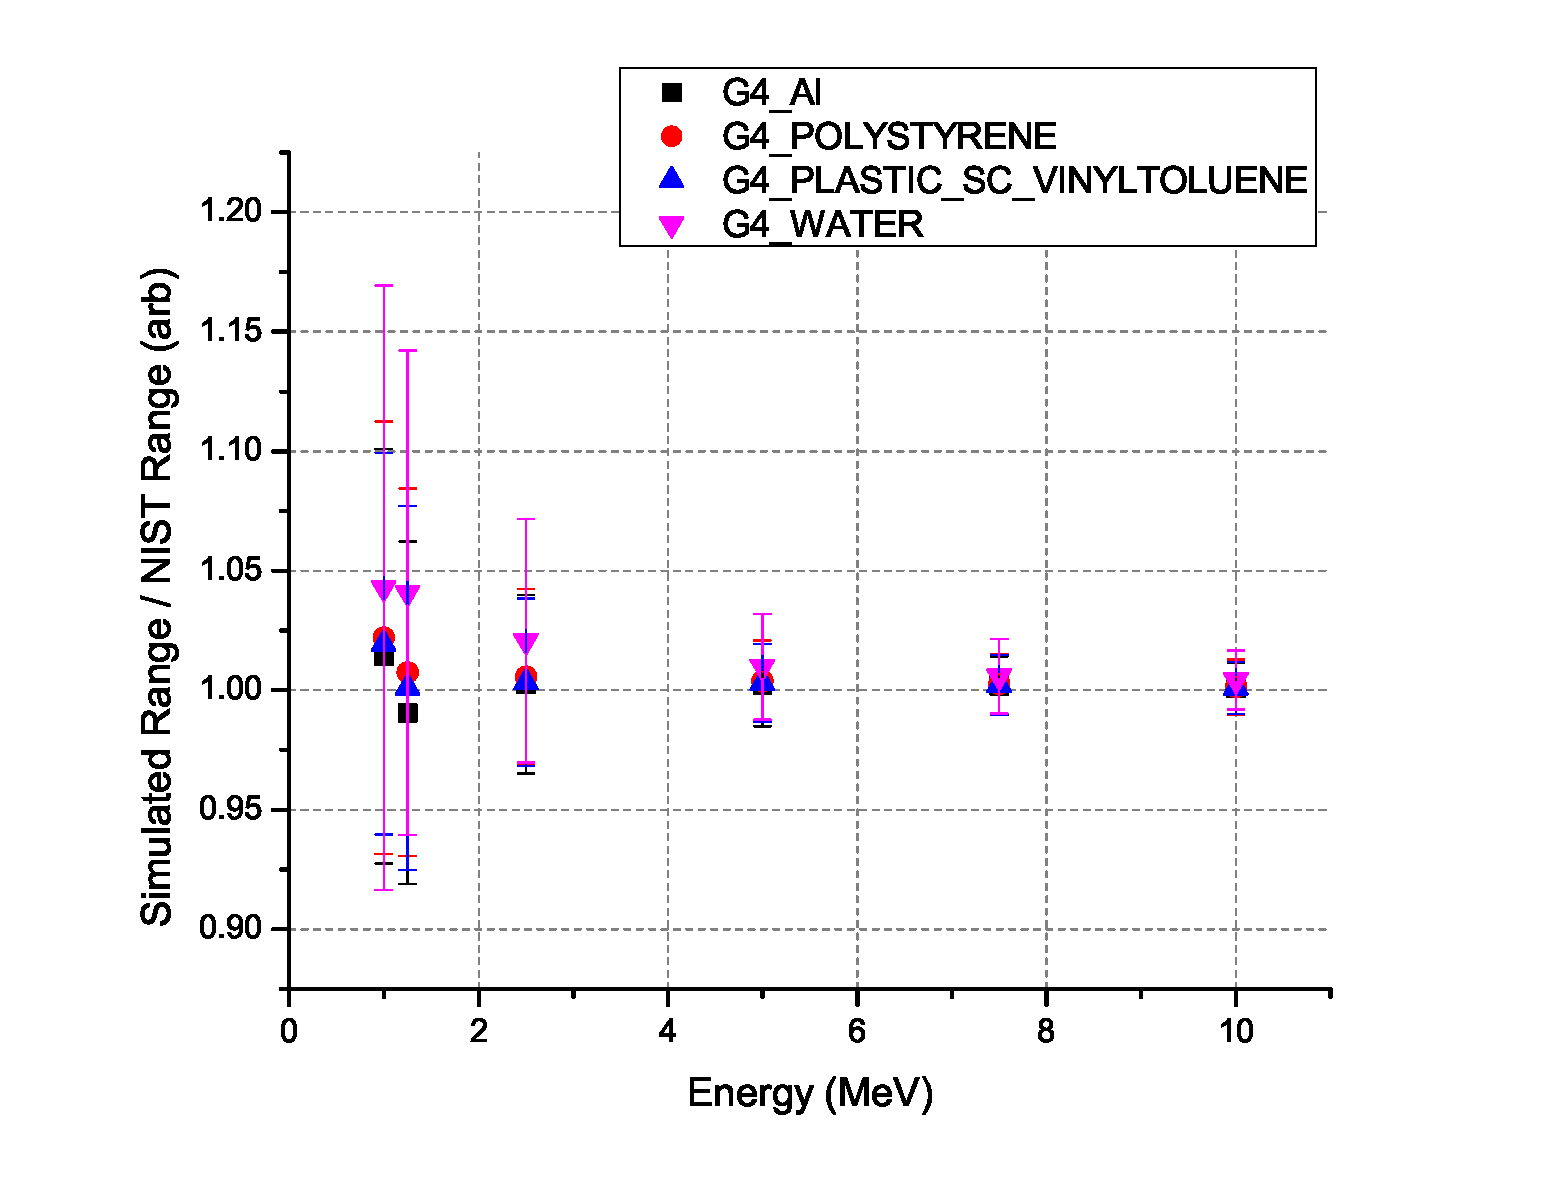
\includegraphics[width=\textwidth]{RangeSim_AlphaVal}
  \caption[Alpha Range Verication]{Comparison of the GEANT4 simulated alpha range to the NIST CSDA range for selected materials.}
  \label{fig:AlphaRangeVal}
\end{figure}
\begin{figure}
  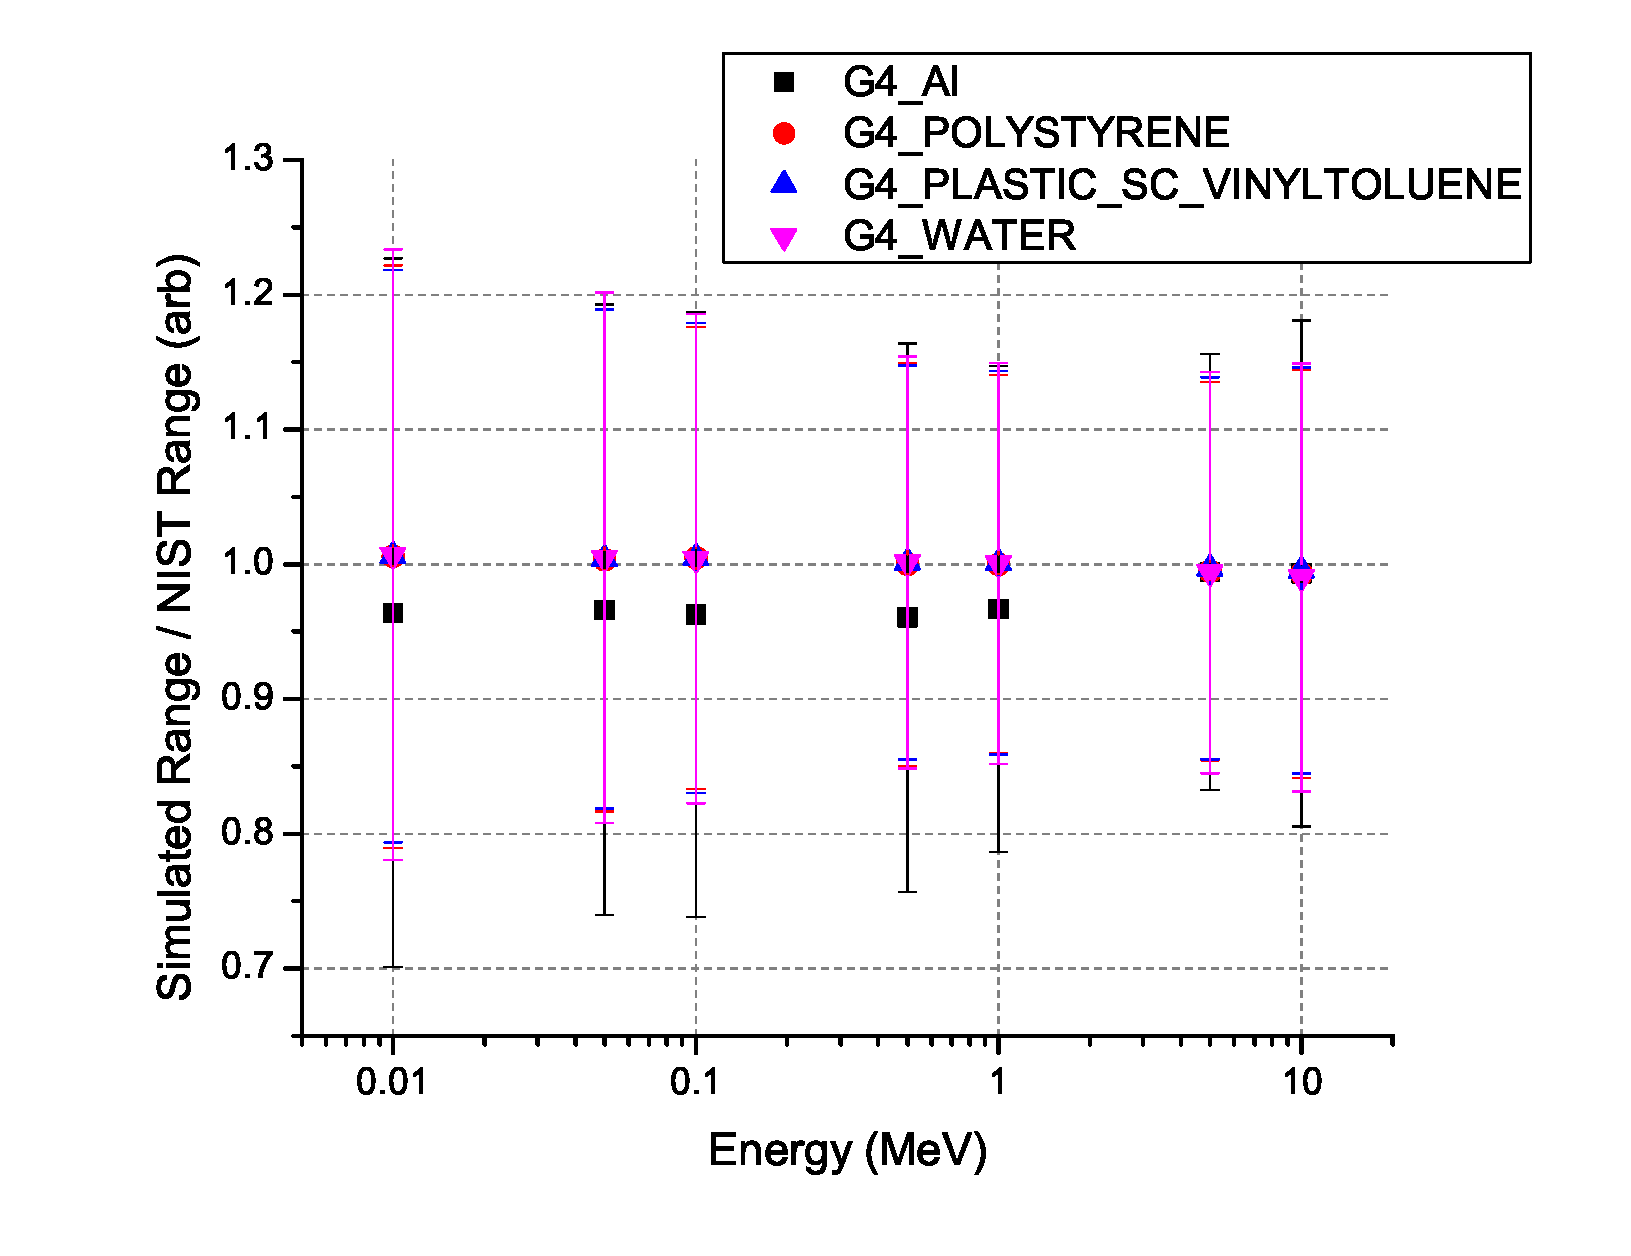
\includegraphics[width=\textwidth]{RangeSim_ElectronVal}
  \caption[Electron Range Verification]{Comparison of the GEANT4 simulated electron range to the NIST CSDA range for selected materials.}
  \label{fig:ElectronRangeVal}
\end{figure}
\autoref{fig:AlphaRangeVal} and \autoref{fig:ElectronRangeVal} show the validation of the alpha and electron ranges, respectively.
It is observed that for alpha particles the simulated range is generally a little bit higher than the NIST range, but for electrons it is less than five precent lower.
Due to the range straggling (indicated by the error bars) it is determined that these small differneces are insignicant, and that the simulation methodology is valid.

The data was compared to the TRIM calculations preformed by Andrew Mabe.
\subsection{Range of Selected Particles and Ions}
\label{sec:RangeResults}

A parametric study was completed on the how the range changes with increasing amount of absorber.
\begin{figure}
  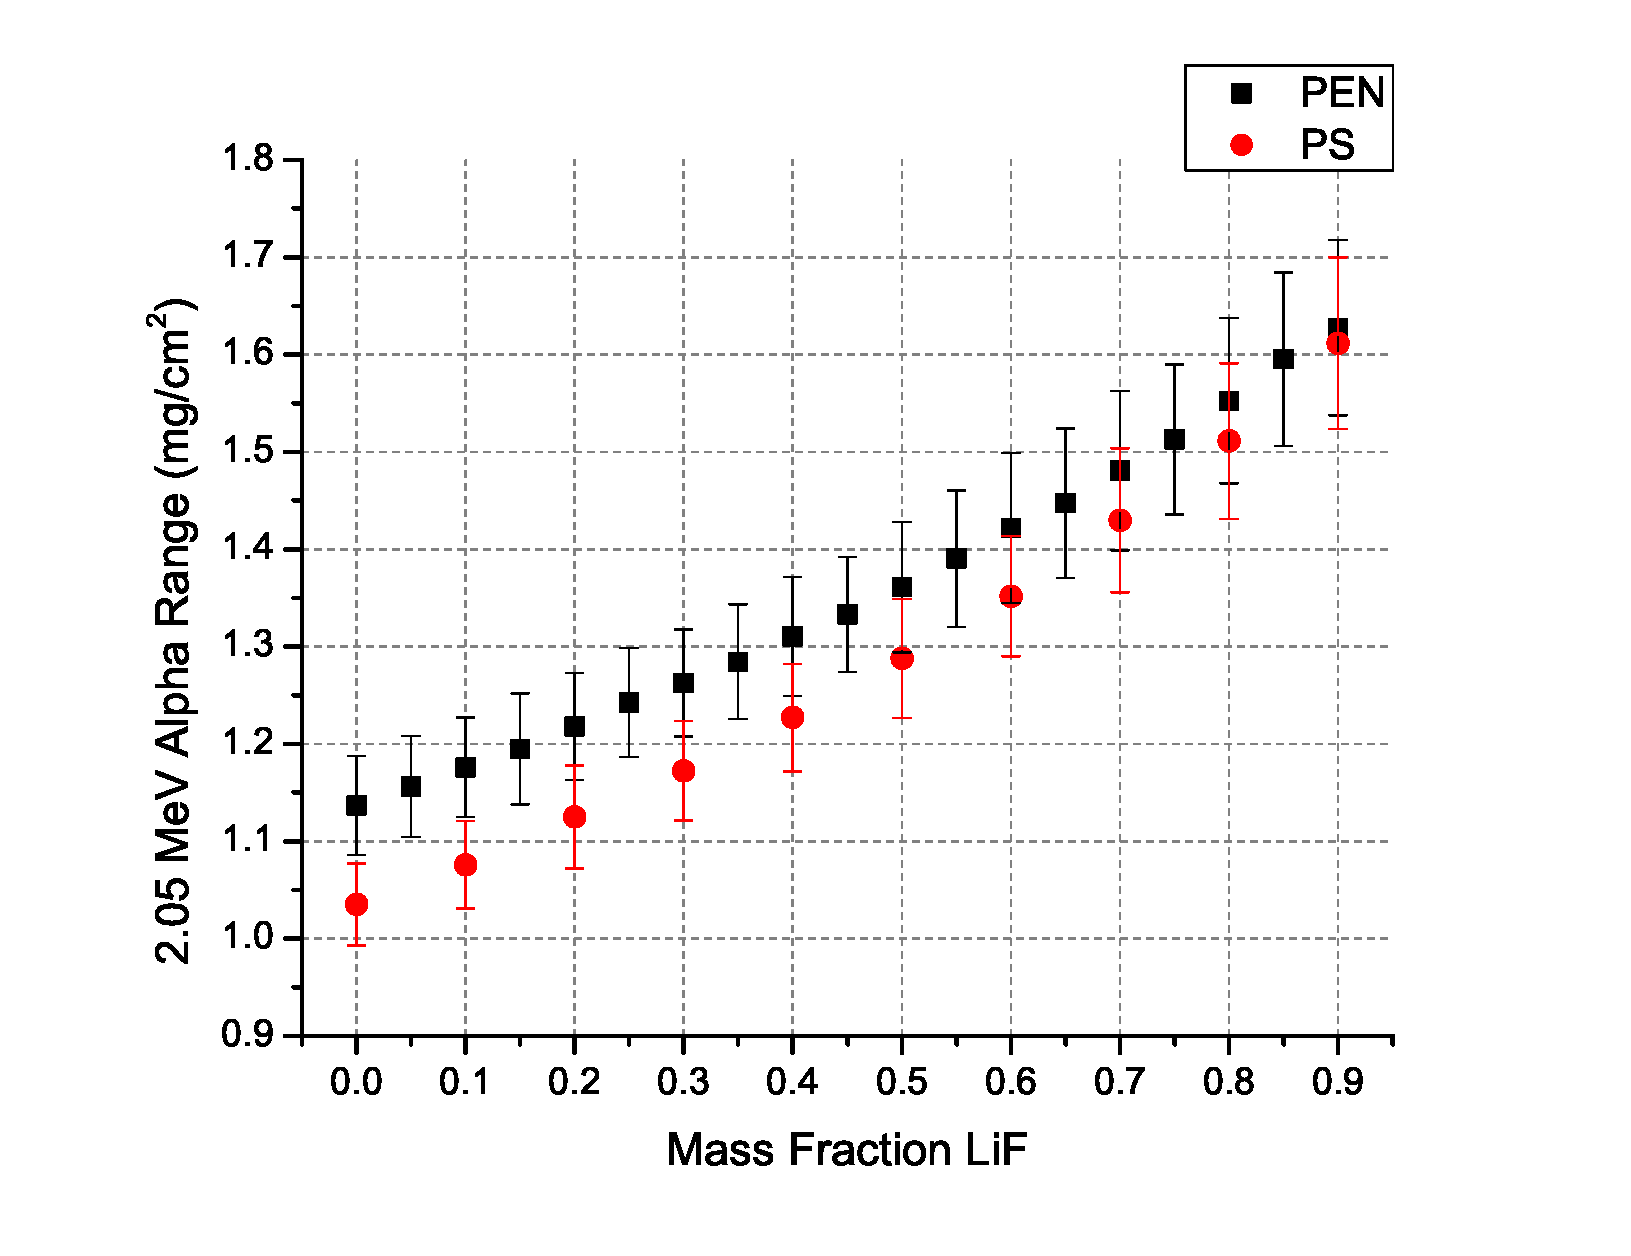
\includegraphics[width=\textwidth]{RangeSim_MassFraction_Alpha}
  \caption[2.05 MeV Alpha Range in PS and PEN Composites]{Range of the \SI{2.05}{\MeV} alpha in PS and PEN LiF loaded films. Initially the ranges are very differnet (due to the differnet ranges in the consituent materials) but as the absorber amount increases the range approaches that of LiF.}
  \label{fig:MassFracRangeAlpha}
\end{figure}
\begin{figure}
  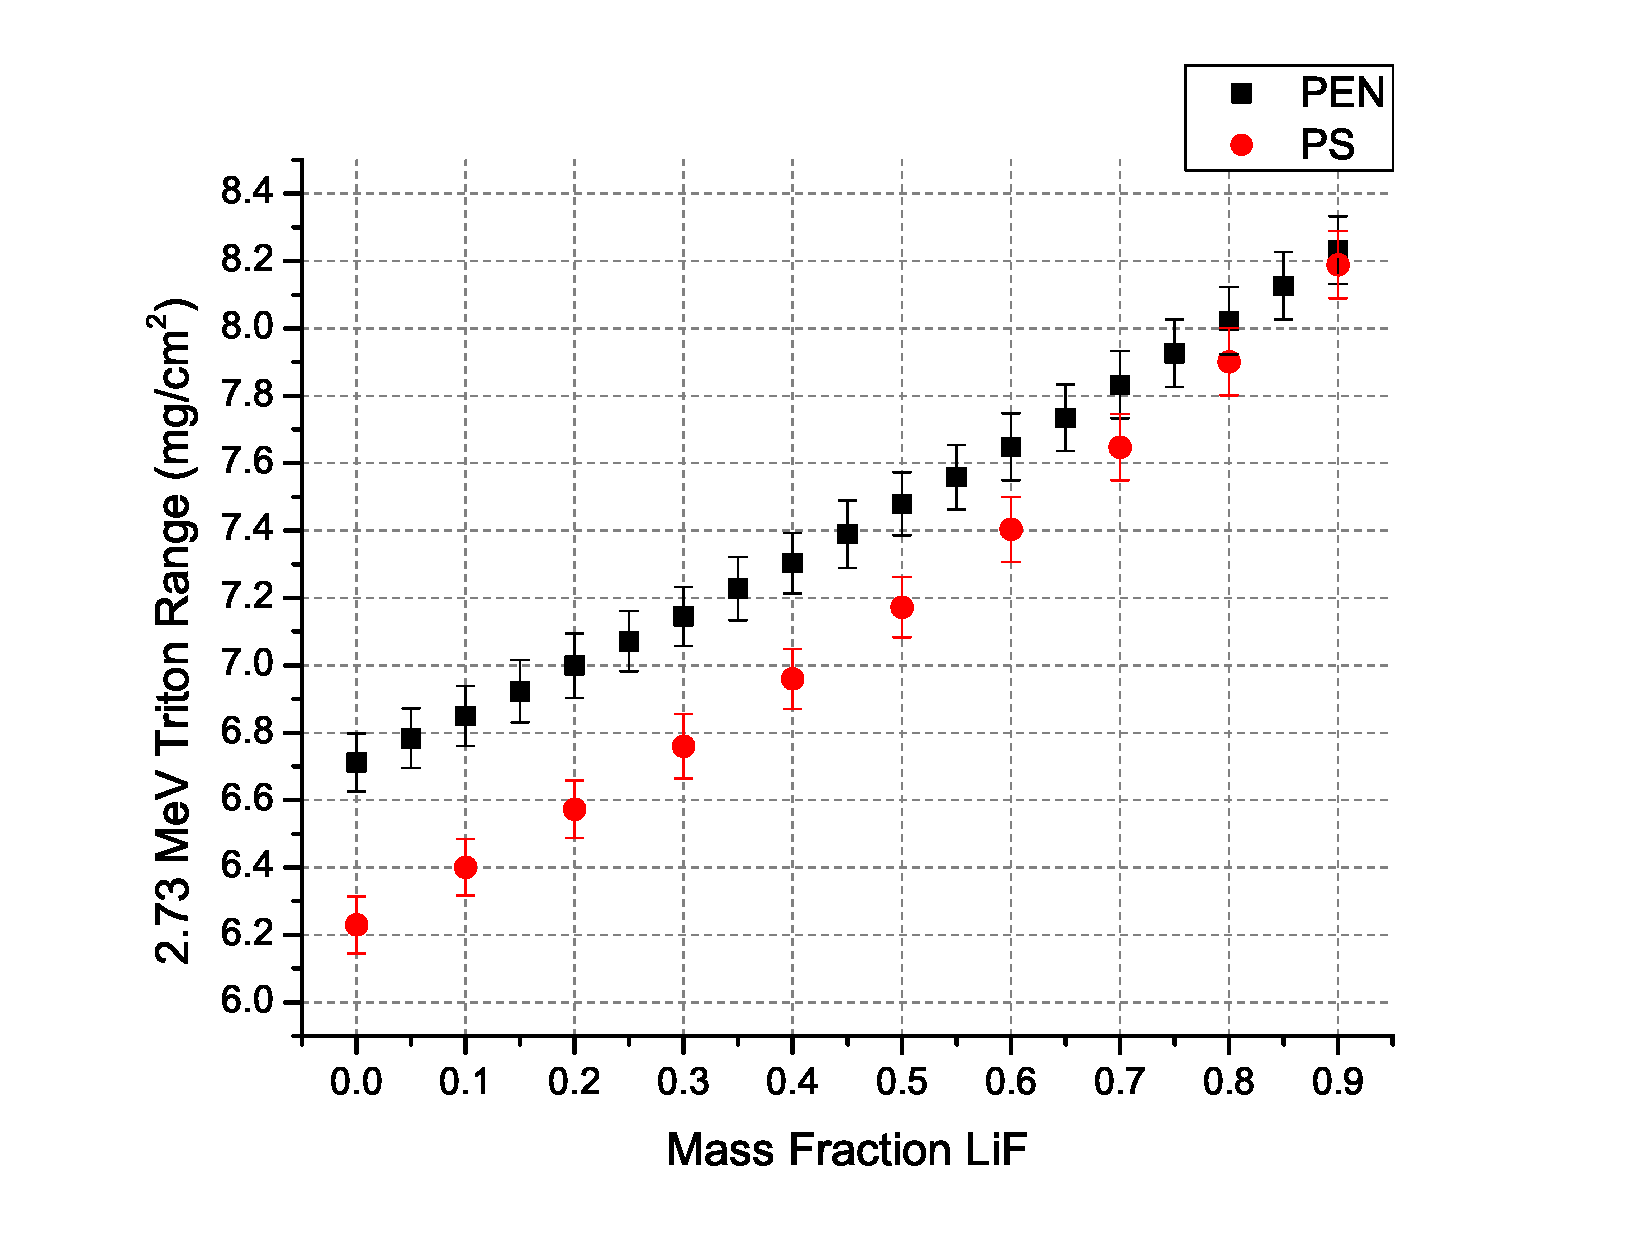
\includegraphics[width=\textwidth]{RangeSim_MassFraction_Triton}
  \caption[2.78 MeV Triton Range in PS and PEN Composites]{Range of the \SI{2.73}{\MeV} triton in PS and PEN LiF loaded films. Initially the ranges are very different, but as the absorber amount increases the range approaches that of LiF.}
  \label{MassFracRangeTriton}
\end{figure}

\appendices
\section{CSDA Range of Lif}
\label{sec:CSDARangeLiF}
\begin{figure}
  \centering
  \begin{subfigure}{0.45\textwidth}
    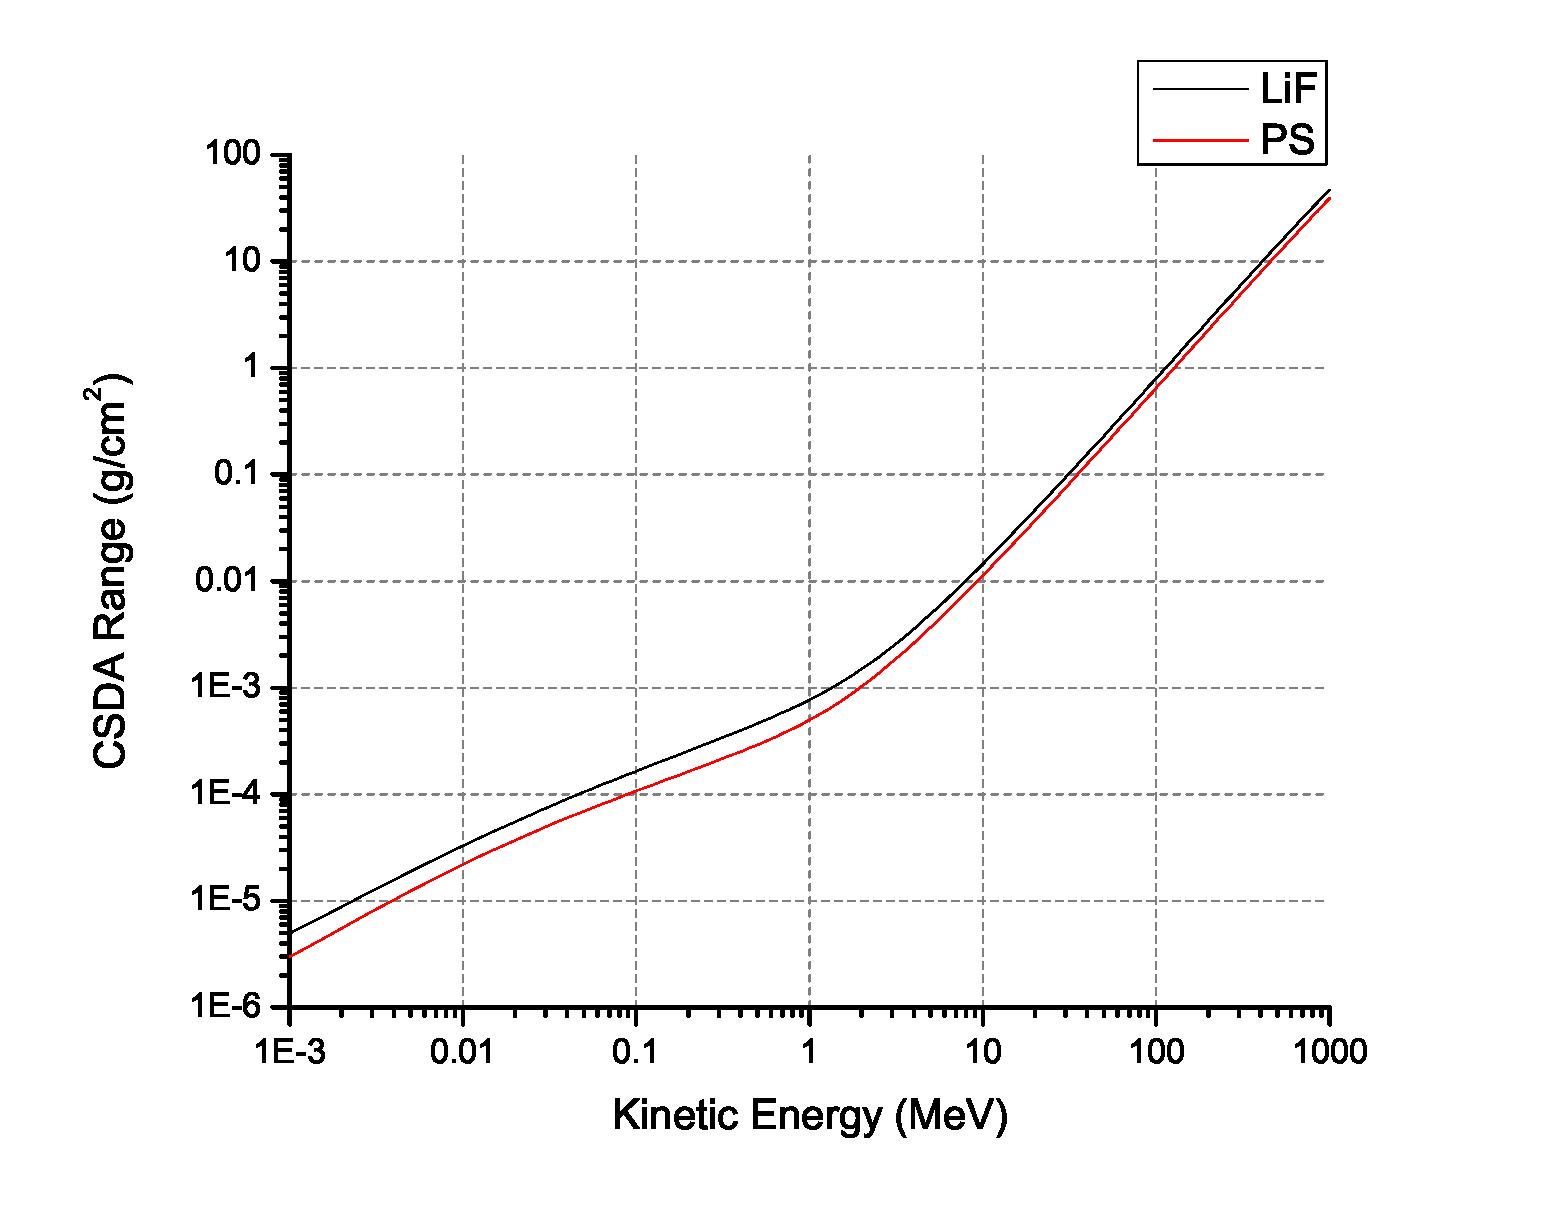
\includegraphics[width=\textwidth]{RangeSim_CSDA-NIST_PS_LiF_rho}
    \caption{CSDA Range shown as surface density}
    \label{fig:NISTPSLiF_rho}
  \end{subfigure}%
  \begin{subfigure}
    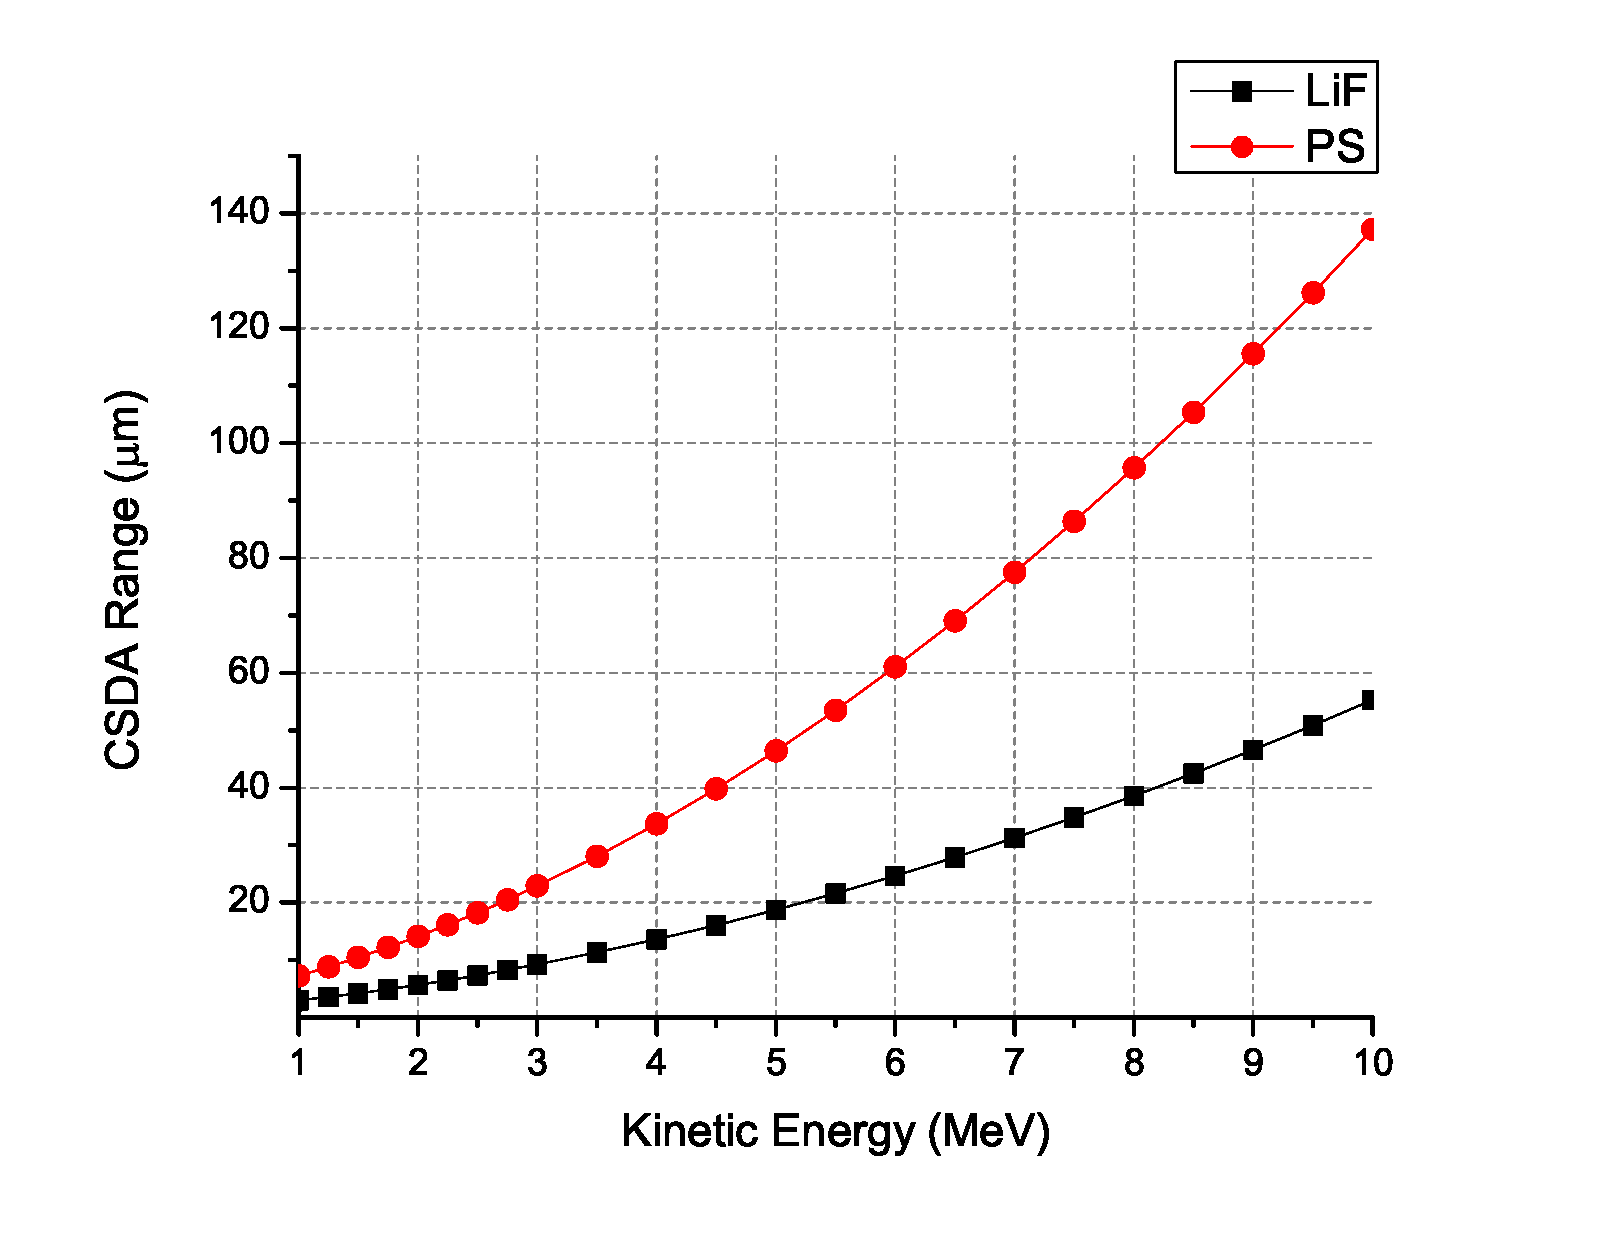
\includegraphics[width=\textwidth]{RangeSim_CSDA-NIST_PS_LiF_um}
    \caption{CSDA Range shown as estimated length}
    \label{fig:NISTPSLiF_um}
  \end{subfigure}
  \caption[Comparison of alpha ranges in LiF and PS]{Comparison of alpha CSDA ranges in PS and LiF. LiF generally has a higher range than PS. Data from NIST ASTAR\cite{berger_estar_2005}.} 
  \label{fig:NISTPSLiF}
\end{figure}

\section{Proton, Deuteron, Triton and Alpha Ranges}
\label{sec:PDTA}
The range of protons, deutrons, tritons, and alpha particles was investigated in water and silicon.
For the same kinetic energy, it is observed that the protons have the largest range, followed by the deutron, triton, and alpha.
This follows the rough relationship described as
\begin{align}
  R_d(E) = 2 R_p\left(\frac{1}{2}E\right)
  
\end{align}
\begin{figure}
  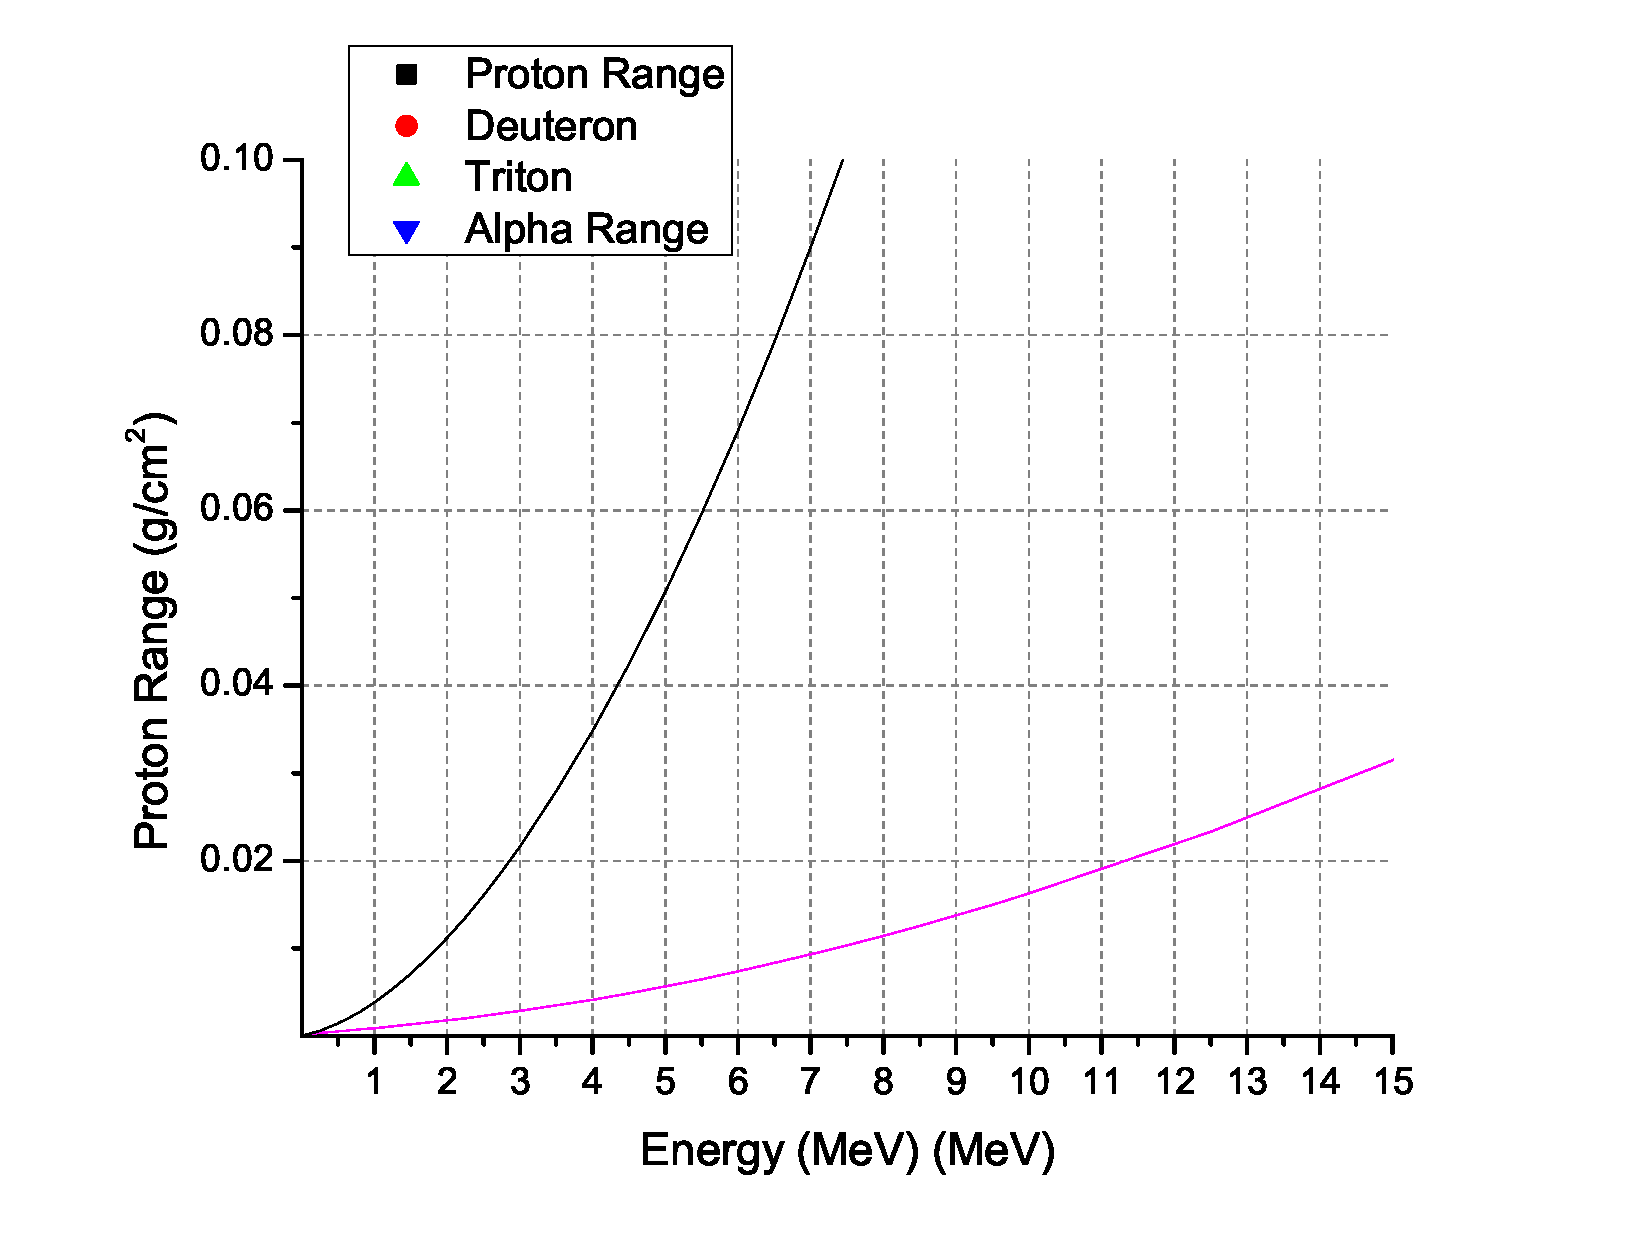
\includegraphics[width=\textwidth]{RangeSim_PDTA_Si}
  \caption[CSDA Range for Differnet Charged Particles in Si]{CSDA Range for protons, deuterons, tritons and alpha in silicon}
  \label{fig:CSDARangePDTASi}
\end{figure}
\begin{figure}
  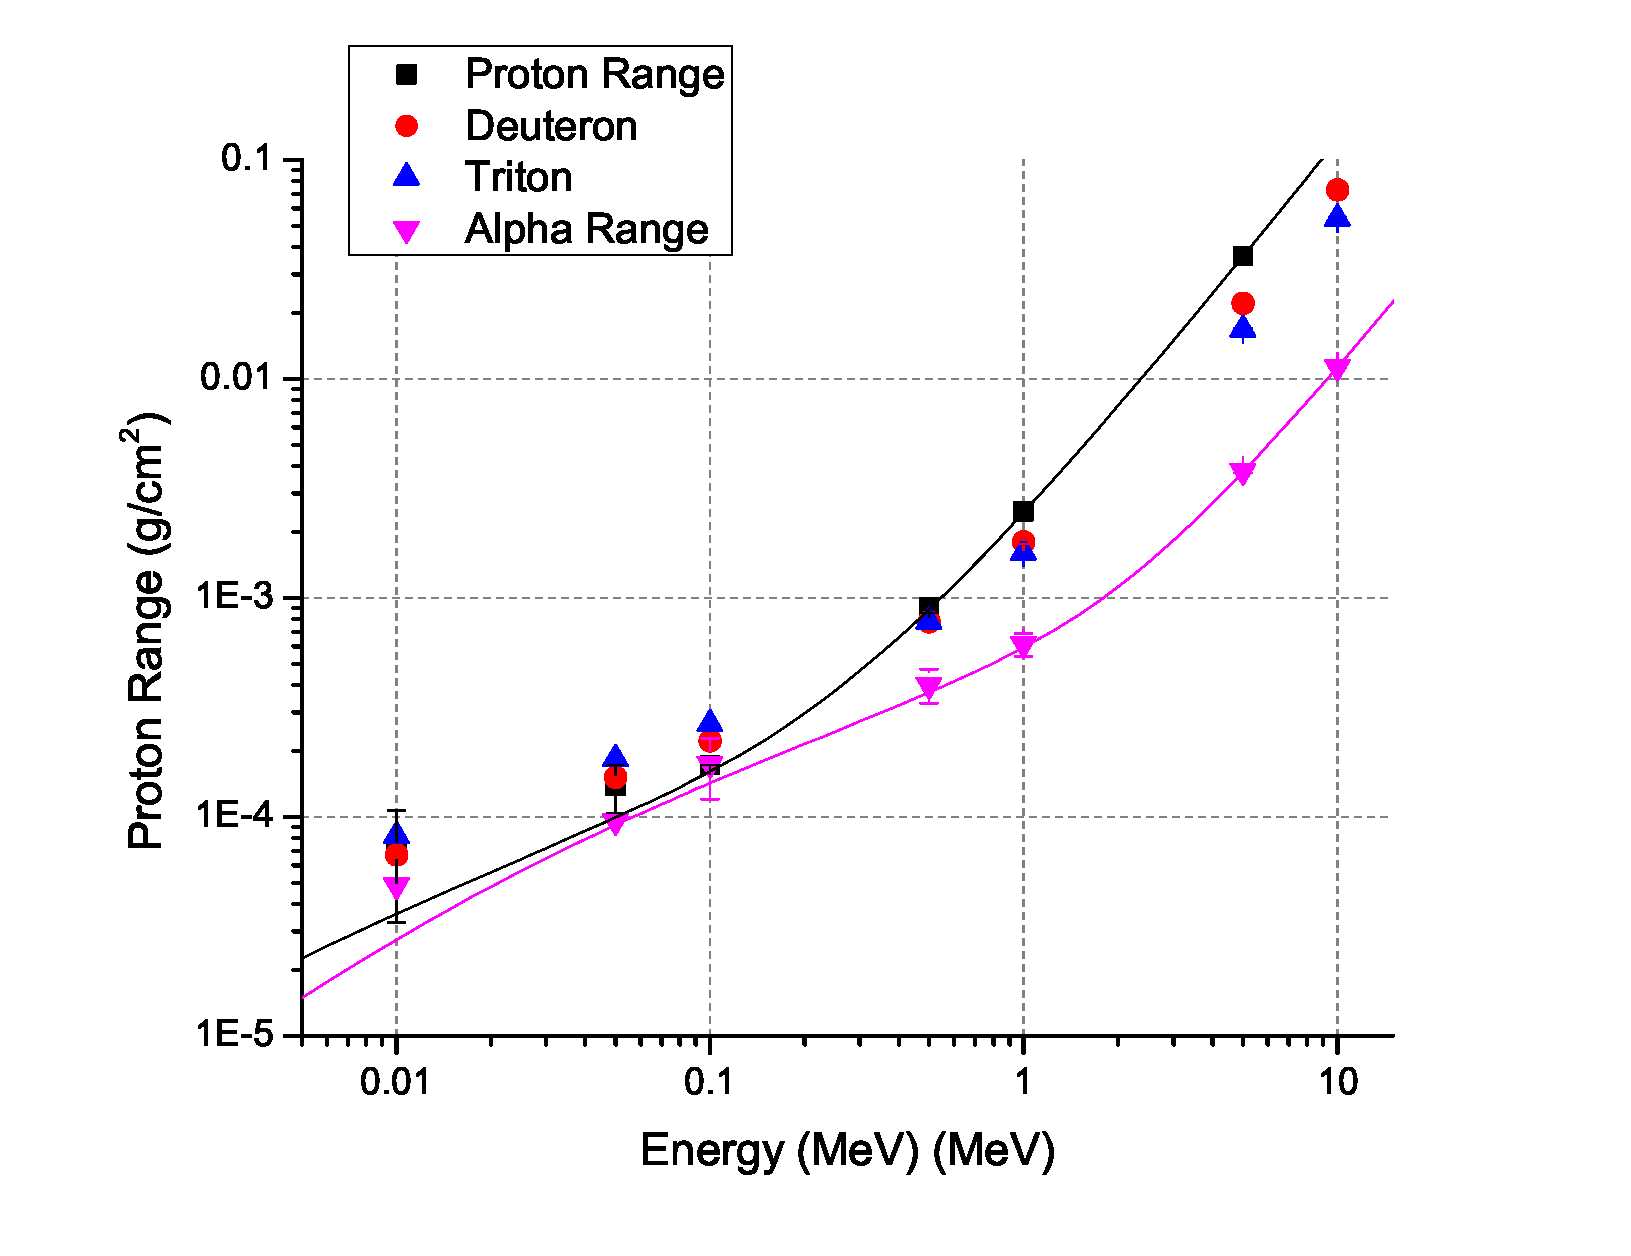
\includegraphics[width=\textwidth]{RangeSim_PDTA_Water}
  \caption[CSDA Range for Differnet Charged Particles in Water]{CSDA Range for protons, deuterons, tritons and alpha in water}
  \label{fig:CSDARangePDTAWater}
\end{figure}

\section{File Locations and Report Status}
The data generated in this report is from a GEANT4 simulation that can be found (at revision 771) \path{https://murphs-code-repository.googlecode.com/svn/trunk/G4/RangeSim}, and the plots were generated with the OriginPro project \path{RangeSim.opj}.
This document is may be found in \LaTeX format at \url{\svnkw{HeadURL}}.  
The latest revision for this file is \svnrev, and was on \svndate, committed by \svnauthor.
\end{document}

